% !TEX encoding = UTF-8 Unicode 
% !TEX root = praca.tex

\subsection{Research scenario 1 results analysis}

The following figures illustrate the aggregated results from the experiments conducted within Research scenario 1 described in Chapter \ref{chap:research_scenarios}.

\begin{figure}[H]
    \begin{minipage}{.48\textwidth}
        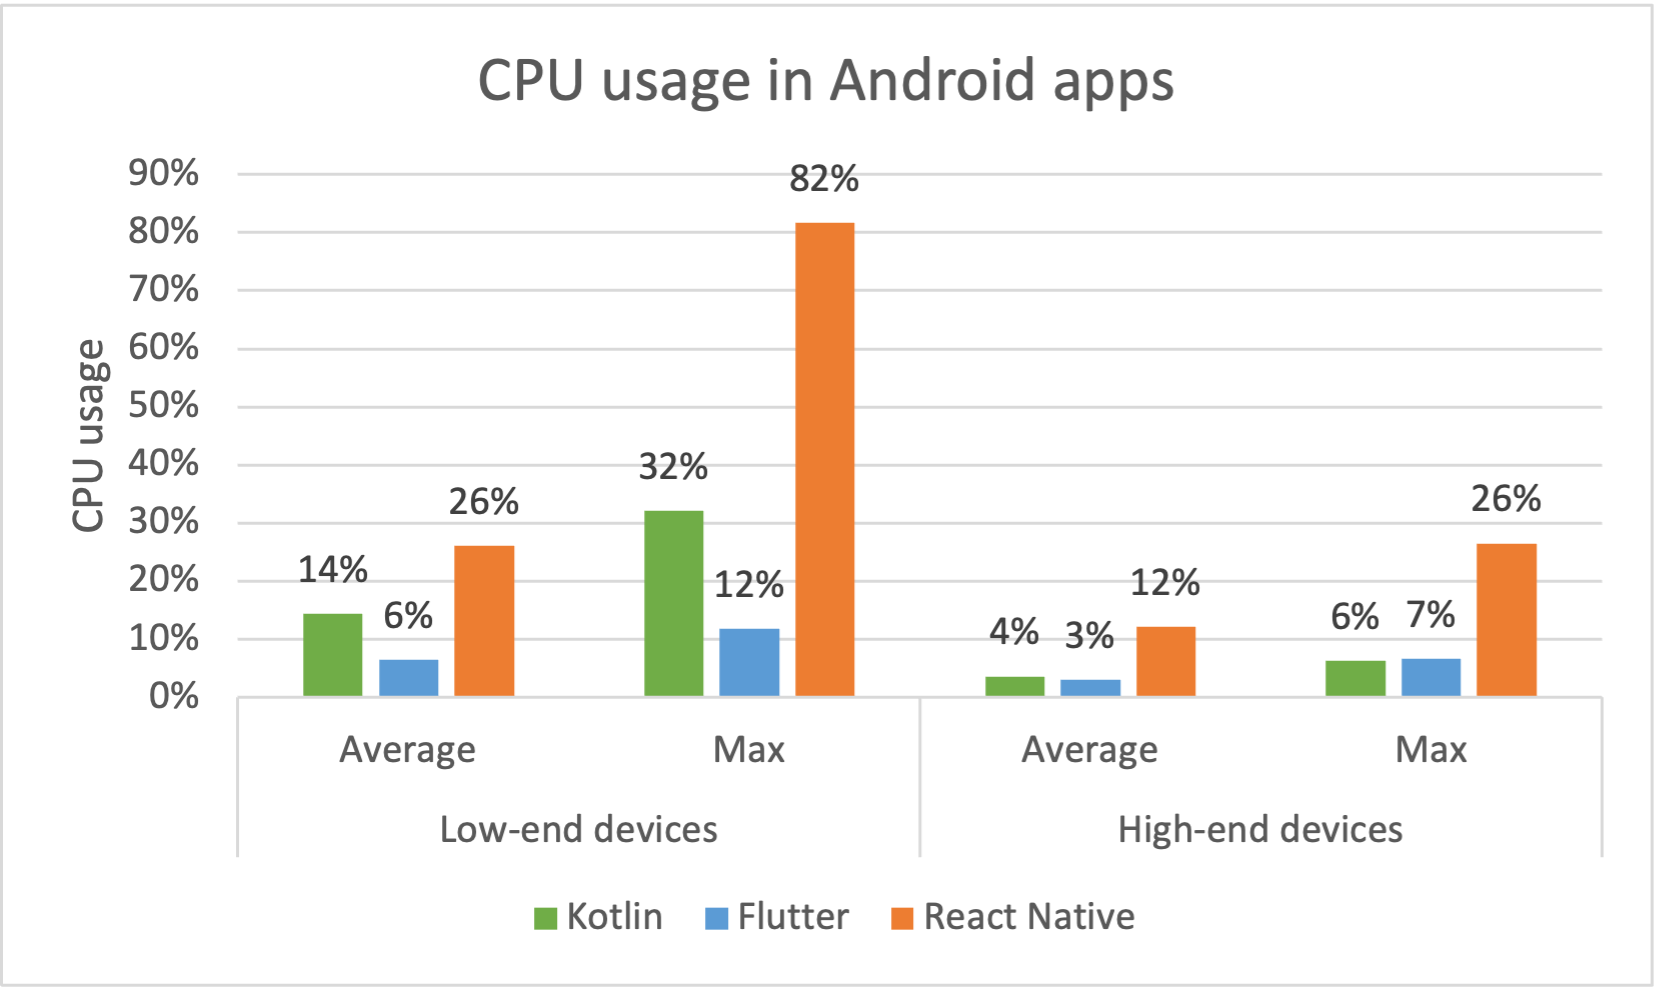
\includegraphics[width=\textwidth]{img/scenario1_cpu_android}
        \caption{Research scenario 1: CPU usage in Android apps (Source: Own work)}
        \label{fig:s1_cpu_android}
    \end{minipage}
    \hfill
    \begin{minipage}{.48\textwidth}
        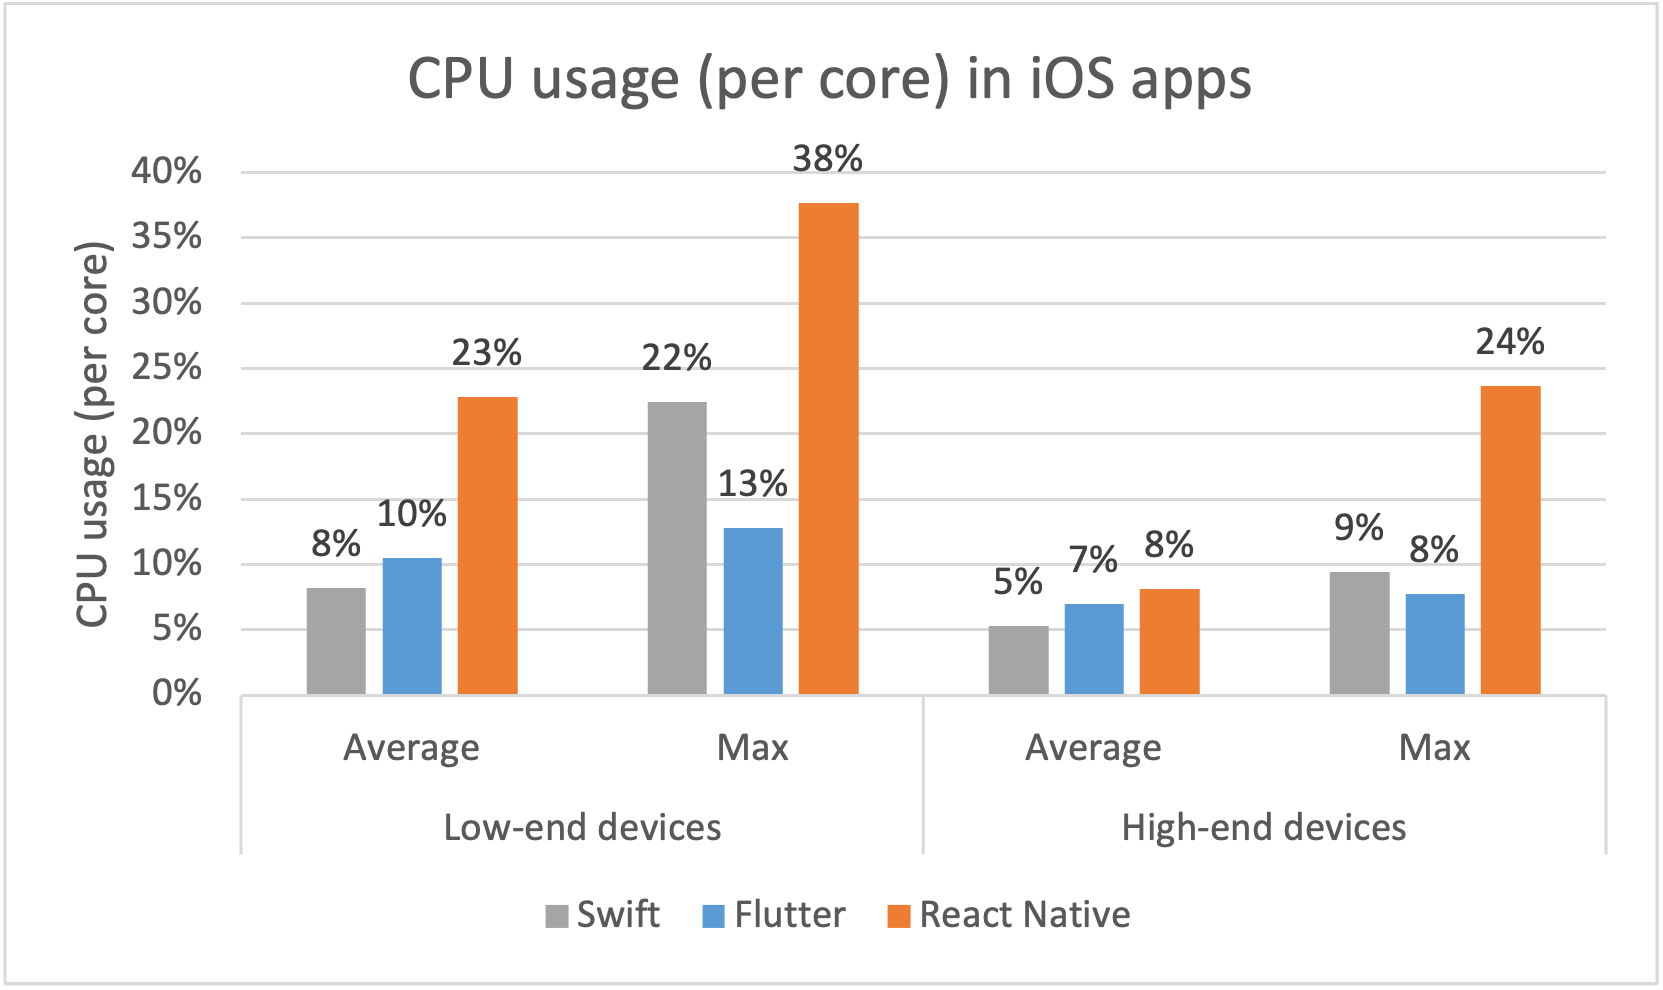
\includegraphics[width=\textwidth]{img/scenario1_cpu_ios}
        \caption{Research scenario 1: CPU usage in iOS apps (Source: Own work)}
        \label{fig:s1_cpu_ios}
    \end{minipage}
\end{figure}

Figures \ref{fig:s1_cpu_android} and \ref{fig:s1_cpu_ios} show the comparison of CPU usage among Android and iOS apps developed with Kotlin, Swift, Flutter, and React Native. For Android apps, Flutter offers the best performance, especially on low-end devices. Kotlin apps utilize 14\% of CPU capacity on average, which is almost two times less than React Native apps (26\%). React Native is again subject to the highest spikes, reaching a maximum of 82\% on low-end devices. On high-end devices, Flutter and Kotlin are on par, while React Native requires moderately more system resources. In the case of iOS apps, native apps developed with Swift demonstrate comparable CPU usage to Flutter apps on both low-end and high-end devices. Again, Flutter experiences the smallest spikes, while React Native exhibits the highest average CPU load combined with the most significant spikes.

\begin{figure}[H]
    \begin{minipage}{.48\textwidth}
        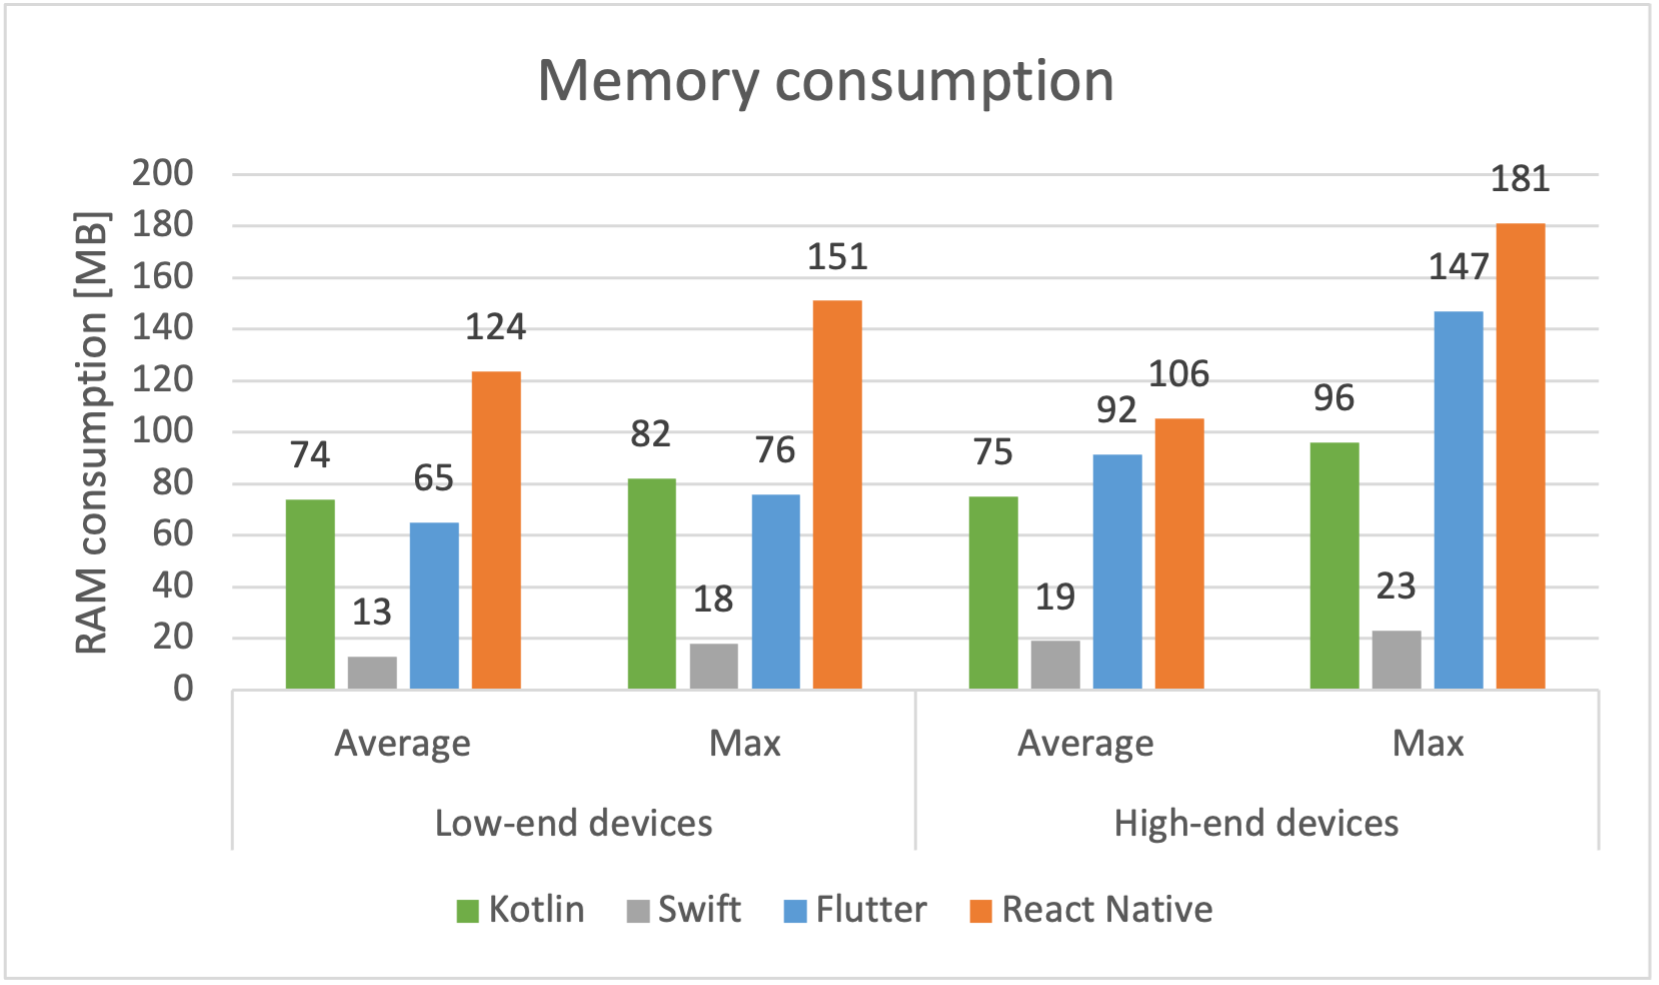
\includegraphics[width=\textwidth]{img/scenario1_ram}
    \caption{Research scenario 1: Memory consumption (Source: Own work)}
    \label{fig:s1_ram}
    \end{minipage}
    \hfill
    \begin{minipage}{.48\textwidth}
        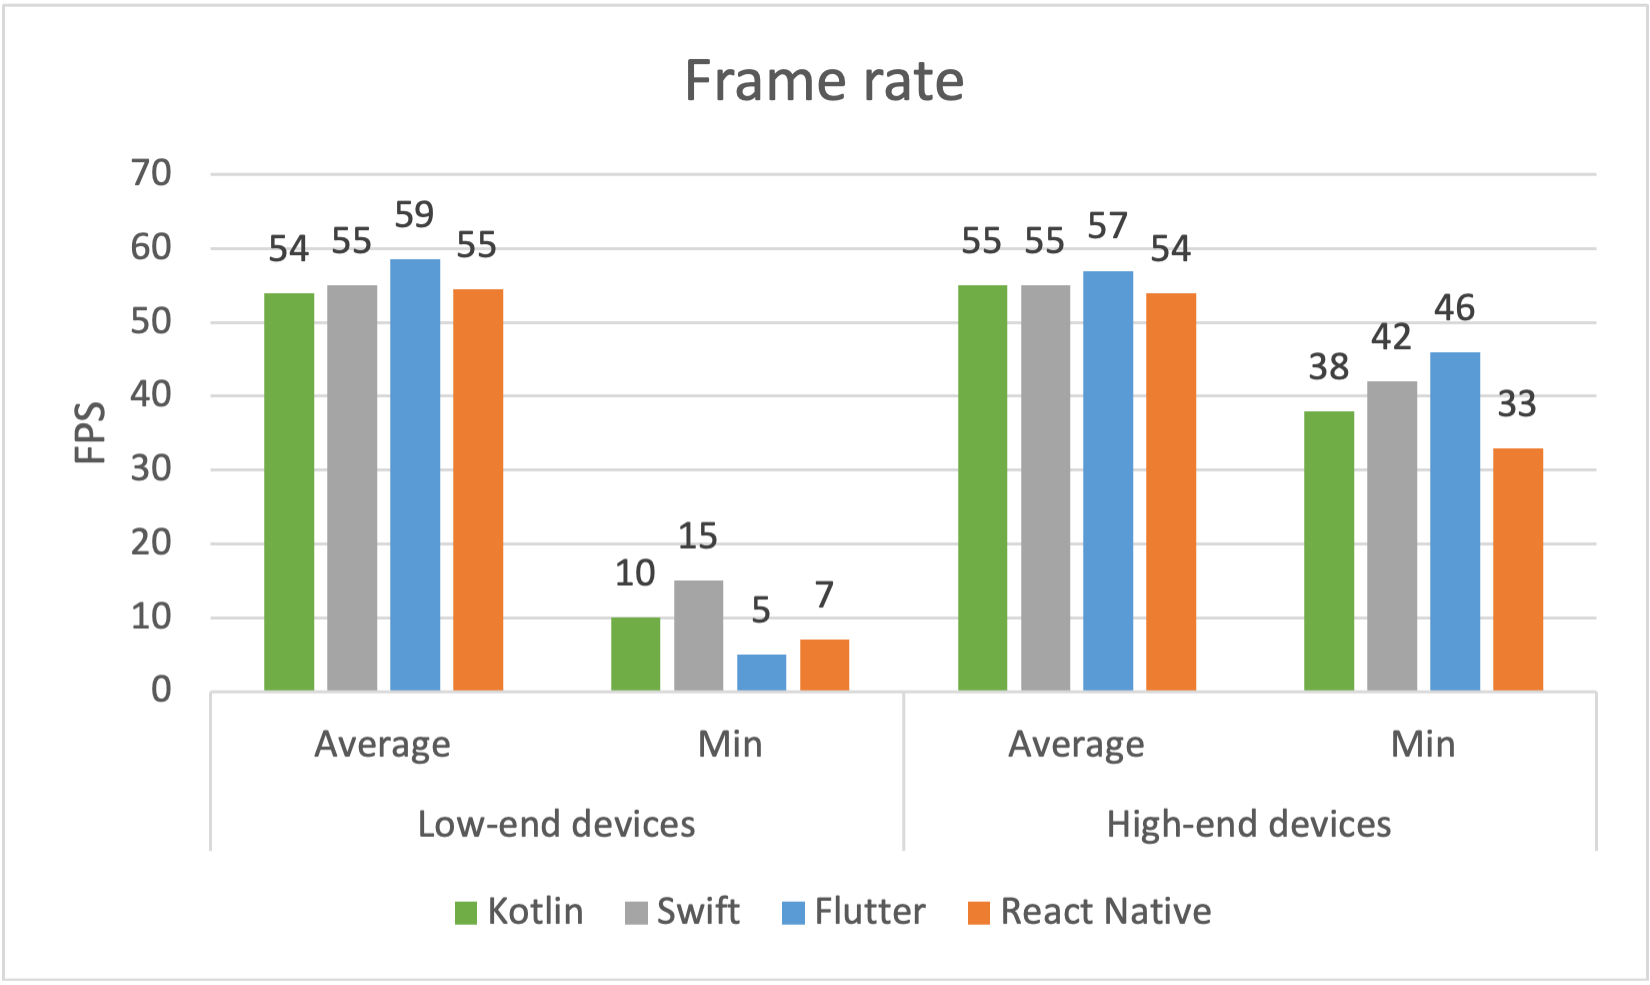
\includegraphics[width=\textwidth]{img/scenario1_fps}
    \caption{Research scenario 1: Frame rate (Source: Own work)}
    \label{fig:s1_fps}
    \end{minipage}
\end{figure}

Figure \ref{fig:s1_ram} shows the comparison of memory consumption among Android and iOS apps developed with Kotlin, Swift, Flutter, and React Native. It can be observed that Swift apps demonstrate the lowest memory consumption on all types of devices compared to other technologies. Flutter apps exhibit similar memory usage, with the latter experiencing higher spikes on high-end devices. React Native apps, on the other hand, perform moderately worse on low-end devices, slightly worse on high-end devices and suffer from bigger spikes.

\bigskip

Figure \ref{fig:s1_fps} show the comparison of frame rate among Android and iOS apps developed with Kotlin, Swift, Flutter, and React Native. In general, none of the technologies suffer from low frame rate on average. However, all of them experience sporadic FPS drops to as little as 5 FPS on low-end devices. Flutter seems to offer the highest overall smoothness with the best result on average and the highest minimum of 46 FPS on high-end devices.
